\documentclass[../report.tex]{subfiles}
\begin{document}

\subsection{Frequency Analysis}
	Another option for analysing the stream was to disregard the amplitudes and concentrate on the frequency domain.  That is to convert to a function of frequency against time.
	
	Many of the frequencies that occur within the streams are considered noise, especially those of a higher frequency that are likely caused by wind so again a Butterworth Bandpass \citep{bandpass} was applied eliminating frequencies outside of the 1-20Hz range.  Code was then written to interpolate the modulation in frequency by means of differentiating the phase inversions.  The code consisted of three functions, \textit{frequency}, \textit{phase\_inversions} and \textit{zero\_intersect}.
	
	The \textit{frequency} function takes two parameters, the first being a series (or array) of observation values and the second being the interval in millisecods between the observations (it assumes evenly timed datapoints).  The series is fed through the phase inversions function that scans the series for the value moving from positive to negative or vice versa.  When it finds an inversion, it passes the Z values from either side of the inversion to \textit{zero\_intersect} which liniearly interpolates the point at which it crossed the x-axis.  This is the passed back up to the frequency function which divides 500 (to convert a half cycle in milliseconds to cycles per second) by the distance between the two observations to estimate the frequency and returns this value along with the midpoint between the timestamps.
	
	The results of this for four events recorded at four stations are shown below (events in columns, stations in rows with the x-axis being the time in milliseconds since the detected start and the y-axis showing interpolated frequency in Hz.)

\begin{figure}[H]
	\centering
	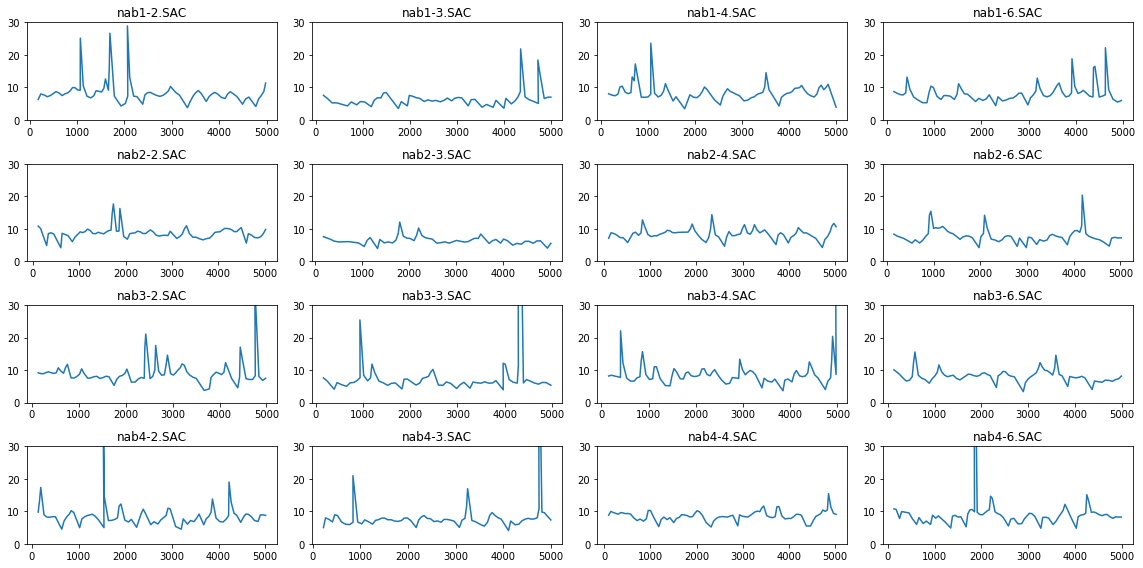
\includegraphics[width=1\linewidth]{img/freq_anal}
	\caption{Interpolated Freqencies}
	\label{fig:freq_anal}
\end{figure}

	As when looking at the amplitudes in \cref{sec:sampledata}, there is no obvious correlation between the stations for the same event.  It was decided not to investigate further.

\end{document}